\documentclass{article}
\usepackage[utf8]{inputenc}

\title{CS 6K W4 GIT Assignment}
\author{jcastano Castanon Remy}
\date{September 2022}

\begin{document}

\maketitle

\section{Myself}

During my experience working as a cybersecurity analyst, I have always faced different issue related to the field. I always thought no one had the interest to solve or even address this issues. Common issues that I have found while working are disinformation, disinterest and uncontrol. This constitutes my second goal. I would love to research and solve issues within the cybersecurity field that no one is paying attention to. One of this issues is the fact that many companies that I had the opportunity to work for, all lack a proper inventory of software leading to security issues.



In addition to my goals and expectations, I consider myself to be very creative. I love to paint. I consider myself an artist in multiple disciplines. I love charcoals and pencils. I am currently learning color theory as well as how to paint figurines and build dioramas. Apart from my artistic face, I love biking. It is the best way for me to add cardio to my gym routine without getting bored.

I will be completing my PhD in Cybersecurity.


\begin{figure}[htp]
    \centering
    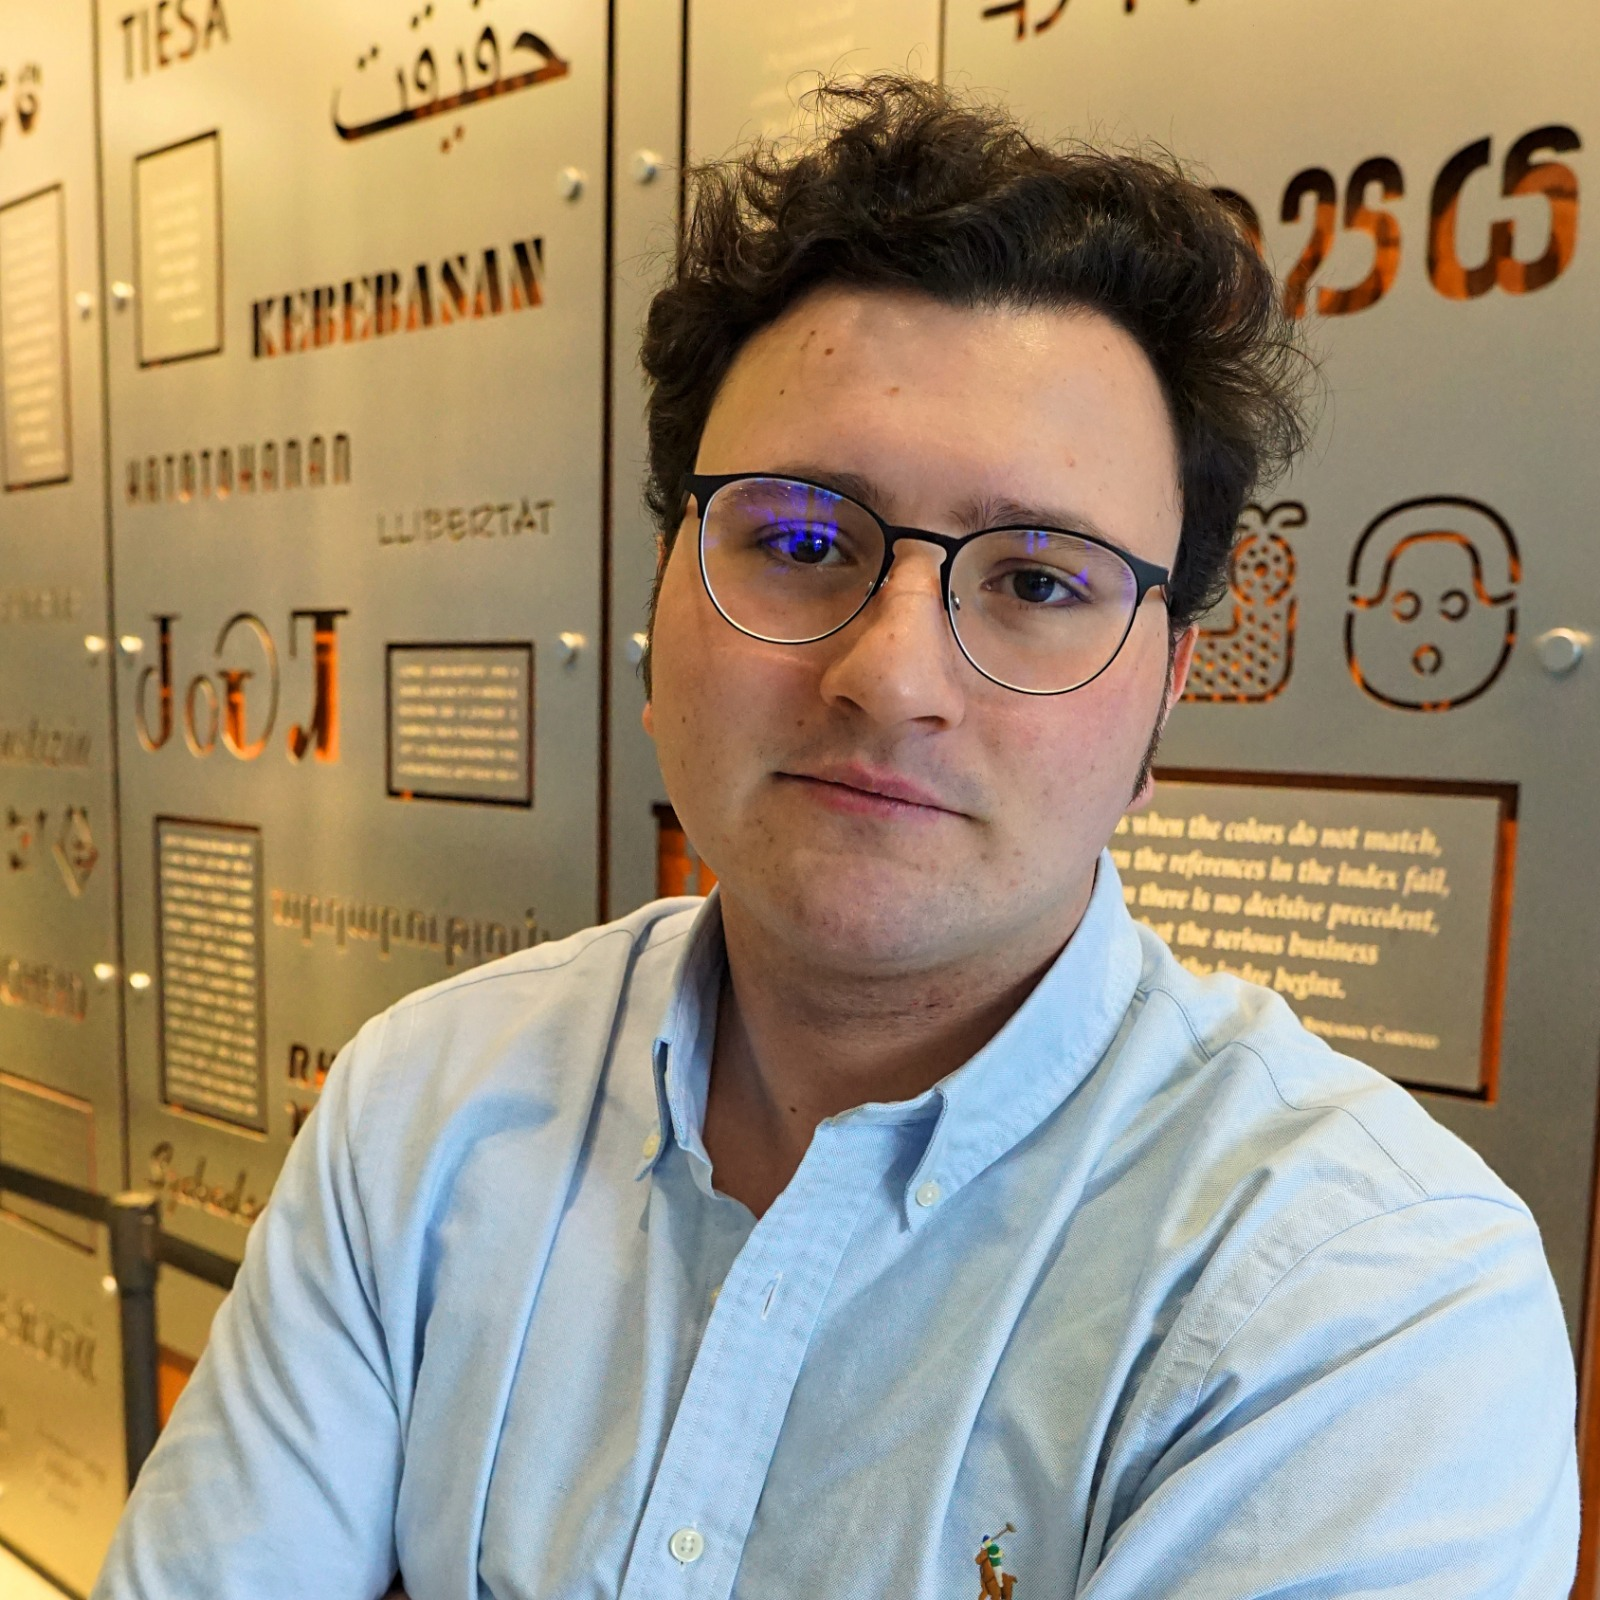
\includegraphics[width=5cm]{UCCSProfileIMG.jpg}
    \caption{An image of myself}
    \label{fig:myself}
\end{figure}


Please, leave your questions after this line.


\end{document}
